\newpage

\section{Details on decomposition analysis}
The decomposition analysis is about proving that the verification of the properties on the sub-models allows the verification of the initial property on the global model. 

The idea of the proof will be illustrated on a row composed of 5 blocks, named $b_1$ to $ b_5 $, as shown in figure~\ref{fig:decompooA}. The duration of each block is greater than the sum of the opening and closing times of the nozzles, which is a necessary assumption given in the step 2 of AMPS. The row is divided into 2 parts: $ P_A $ groups together the first three blocks, and $ P_B $ includes the blocks $ b_3 $ to $ b_5 $. $b_{3}$ is the overlapping block and so is included in both $P_A$ and $P_B$. The decomposition criterion is such that $C_{best}=C_{alt}$. Thus, on the block $b_3$ for which overlapping occurs, the command is known.


\begin{figure}[h!]
	\begin{center}
		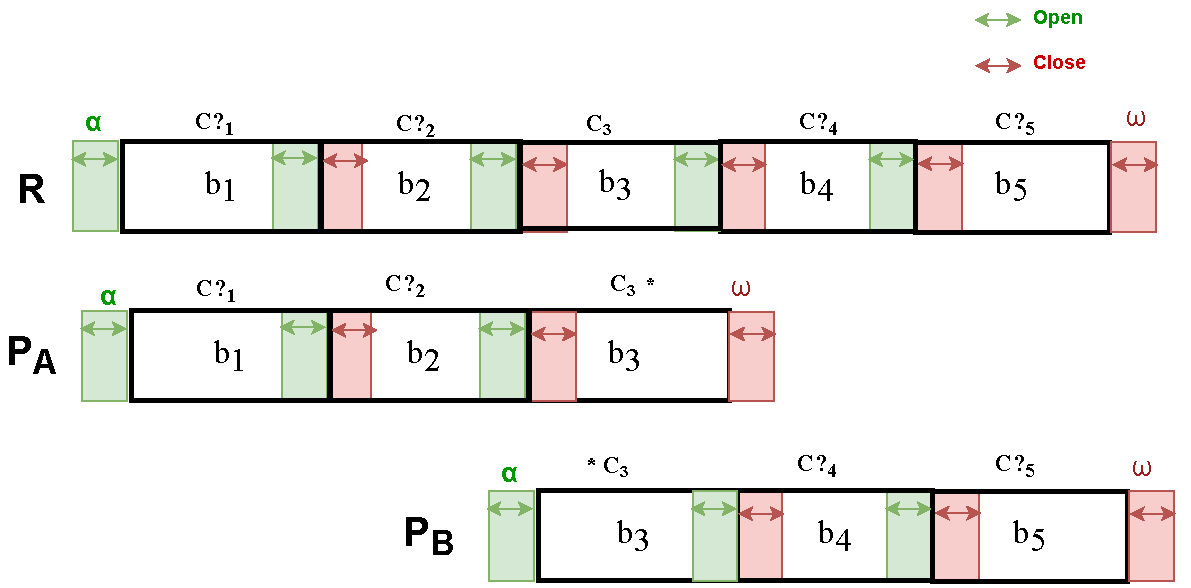
\includegraphics[width=7.2cm]{decompo2.pdf} 
		%\caption{Illustration of the proof of decomposition}
		\caption{Illustration of the decomposition to support proof} 
		\label{fig:decompooA}
	\end{center}
\end{figure} 

For the example row $R$ depicted in figure \ref{fig:decompooA}, a sequence $S_R$ for the whole row can be written:
\begin{equation}
	S_R = C?_{1} \triangleright C?_{2} \triangleright C_{3} \triangleright C?_{4} \triangleright C?_{5}  \label{eq:SRExampleA}
\end{equation} % instead of cmd_{i} 

where $C_{i}$ is the command for block $b_{i}$ when it is unique (as for the overlapping block $b_3$) and where $C?_{i}$ denotes a choice to make for block $b_i$

In order to take into account that, before each row, and at the end of each row, all nozzles should be closed, equation \ref{eq:SRExampleA} rewrites, with $\oslash$ meaning all nozzles off:

\begin{equation}
	S_R = \oslash \triangleright C?_{1} \triangleright C?_{2} \triangleright C_{3} \triangleright C?_{4} \triangleright C?_{5} \triangleright \oslash \label{eq:SRExample_r_anxA}
\end{equation}

Sequences $S_A$ and $S_B$ for parts $P_A$ and $P_B$ can be written:

\begin{eqnarray}
	&S_A =& \oslash \triangleright C?_1 \triangleright C?_2 \triangleright C_{3}* \triangleright \oslash \label{eq:SAExample_r_anxA}
	\\
	&S_B =& \oslash \triangleright *C_{3} \triangleright C?_4 \triangleright C?_5 \triangleright \oslash \label{eq:SBExample_r_anxA}
\end{eqnarray}

The symbol $*$ either on the left or on the right of $C_3$ denotes that overlapping occurs here. 

Details on the costs (product consumed) need now to be given. A rule was enunciated in section \ref{sec:Spraying_Constraints} which can be rephrased in the following way. When changing from one block to another, opening the nozzles needed in the new block and which were closed before has to be anticipated in the end of the previous block. Conversely, the nozzles no longer needed in the new block will be closed at the beginning of the new block. The consequences of this rule were explained in figure \ref{fig:CbestCalt} and section \ref{sec:InterestCalt}. The costs  for opening a nozzle $X$ ($Open(X)$), using a nozzle $X$ on a bloc $b_i$ ($Q_i(X)$), and closing a nozzle $X$ ($Close(X)$) were also introduced in section \ref{sec:InterestCalt}.

Let now $C_i$ be a command used for a block $b_i$ which can be defined as a set of opened nozzles. This set $C_i$ is any subset of $\Omega=\{LH,CH,HH\}$ with a cardinal inferior or equal to 2, including the null set $\emptyset$ (for missing vegetation blocks and outside rows).

The cost $Q_i(C_i)$ of using the nozzles of command $C_i$ during block $b_i$ can be written:
\begin{equation}
	Q_i(C_i)=\sum\limits_{X \in C_i} Q_i(X)
\end{equation}

The cost $c(C_i,C_j)$ of changing from one command $C_i$ to a command $C_j$ in the next block may be decomposed in:

\begin{eqnarray*}
	c(C_i,C_j)=open(C_i,C_j)+close(C_i,C_j)\\
	open(C_i,C_j)\ \ = \sum\limits_{X \in Cj\backslash C_i \cap C_j} Open(X) \\
	close(C_i,C_j) = \sum\limits_{X \in Ci\backslash C_i \cap C_j} Close(X)
\end{eqnarray*}

Costs of sequences can now be calculated. The cost $c(S)$ of a sequence $S= C_{i-1} \triangleright C_i \triangleright C_{i+1}$ is the following: 
\begin{equation}
	c(S)=Q_{i-1}(C_{i-1})+c(C_{i-1},C_i)+Q_i(C_i)+c(C_i,C_{i+1})\\+Q_{i+1}(C_{i+1})
\end{equation}

The costs for the start ($\alpha = \oslash \triangleright C$) and the end ($\omega = C \triangleright \oslash$) of a part or of a row are:

\begin{eqnarray}
	c(\alpha) = open(C) + Q(C) \label{eq:costalphaA}
	\\
	c(\omega) = Q(C) + close(C) \label{eq:costomegaA}
\end{eqnarray}

The concatenation law for parts having an overlapping and the rectification terms for costs of concatenated parts can now be formulated. Considering the example of figure \ref{fig:decompooA} and the sequences provided in equations \ref{eq:SRExample_r_anxA}, \ref{eq:SAExample_r_anxA} and \ref{eq:SBExample_r_anxA}, it follows that:

\begin{equation}
	S_R = S_A \triangleright S_B \Rightarrow C_{3}* \triangleright \oslash \triangleright \oslash \triangleright *C_{3} = C_{3} \label{eq:concatparts_anxA}
\end{equation}

\paragraph{Concatenation rule for row parts} Considering two row parts overlapping on a block for which command $C$ is known a priori (because $C_{best}=C_{alt}$), the concatenation rule for handling the overlapping block is the one of equation \ref{eq:ruleconcatpartsA}

\begin{equation}
	C* \triangleright \oslash \triangleright \oslash \triangleright *C = C \label{eq:ruleconcatpartsA}
\end{equation}

Considering that there is overlapping at block $b_{3}$ for which command should not be counted twice, and that termination $oslash$ of part $S_A$ and beginning $oslash$ of part $S_A$ are virtual, the concatenation rule stipulated in equation \ref{eq:ruleconcatpartsA} is easily understood.

In order to prove that the concatenation of two optimal sequences found for the parts provided by decomposition of this example is an optimal sequence for the whole row, it is required that no term should be changed in the concatenated sequence for it to be optimal, and it is required to be able to calculate the optimal cost for the whole sequence from the optimal costs of the parts.
Considering the first point, and considering two overlapping sequences such as $S_A$ and $S_B$ from our example. In an optimal choice for $C?_{1}$ and $C?_{2}$ within $S_A$, these choices only depend on the value of $C_{3}$ which is known. The same applies to choices for $C?_{1}$ and $C?_{2}$ within $S_R$. Thus, the optimal choices for $C?_{1}$ and $C?_{2}$ made in solving $S_A$ are still valid for $S_R$. With similar reasoning, it follows that optimal choices for $C?_{4}$ and $C?_{5}$ made when solving $S_B$ are still valid for $S_R$. Thus, provided that the concatenation rule stipulated in equation \ref{eq:ruleconcatpartsA} is applied, the optimal sequence for $S_R$ can be calculated from its $S_A$ and $S_B$ parts. This reasoning extends straightforwardly to calculating the optimal sequence for a vine row using $n$ row parts.
Considering the second point, cost calculation, it can be done from the costs calculated for the parts.

%\begin{equation}
\begin{eqnarray}
	c(S_A) & = & open(C?_{1})+Q_{1}(C?_{1})+c(C?_{1},C?_{2})+Q_{2}(C?_{2})+c(C?_{2},C_3) \nonumber \\*
	& + & Q_{3}(C_{3})+close(C_{3}) \label{eq:costsa_anxA} \\
	c(S_B) & = & open(C_{3})+Q_{3}(C_{3})+c(C_{3},C?_{4})+Q_{4}(C?_{4})+c(C?_{4},C?_{5}) \nonumber \\*
	& + & +Q_{5}(C?_{5})+close(C_{5}) \label{eq:costsb_anxA}
\end{eqnarray}
%\end{equation}

The cost $c(S_R)=c(S_A \triangleright S_B$) can be calculated from the $S_R$ in a similar manner as in equations \ref{eq:costsa_anxA} and \ref{eq:costsb_anxA}. Defining $corr(S_A \triangleright S_B)$ by equation \ref{eq:costcorrection_anxA}, this term can be easily calculated from equation \ref{eq:correctionterm_anxA}

\begin{equation}
	c(S_R)=c(S_A \triangleright S_B)=c(S_A)+c(S_B)+corr(S_A \triangleright S_B) \label{eq:costcorrection_anxA}
\end{equation}

\begin{equation}
	corr(S_A \triangleright S_B)= - Q_{3}(C_{3}) - close(C_{3}) - open(C_{3}) \label{eq:correctionterm_anxA}
\end{equation}

This cost correction easily extends to cost correction for the calculation of optimal cost of a row from optimal sequences on $n$ row parts.
